%\chapter{Recuperación de información: limInfo} \label{append:limInfo}

\begin{center}
    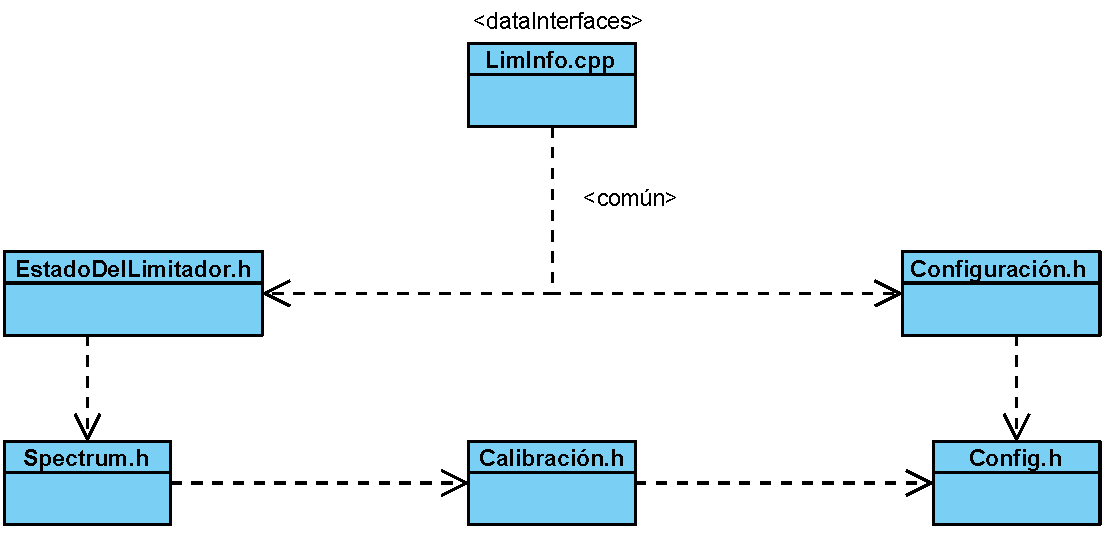
\includegraphics[width=0.9\textwidth]{figuras/lms9-limInfo.pdf}
    \captionof{figure}{Diagrama de dependencias del programa limInfo.}
    \label{fig:limInfo}
\end{center}

El programa recibe como parámetro una cadena de caracteres, en la que cada carácter corresponde a la consulta de una propiedad del limitador. En el listado de códigos de este anexo se muestra la información que exporta el programa \verb|limInfo| y el carácter necesario para su consulta.

En la figura \ref{fig:limInfo} se muestra el diagrama de dependencias del programa. Este diagrama representa la inclusión de otros ficheros de código fuente C++ en el fichero \verb|limInfo.cpp|. Estas inclusiones no siempre son clases, por lo que \textbf{no debe confundirse con un diagrama de clases}. En las relaciones se muestra entre ángulos el módulo al que pertenece (la carpeta en la que se encuentra dentro del proyecto).

Este programa se consideró redundante ya que se puede obtener la misma información mediante el \verb|getConfig|, por lo que no ha sido exportado ni utilizado por nuestro sistema.

Leyenda:
\begin{itemize}
    \item El símbolo igual (=) indica cuál es el valor por defecto de la propiedad a la que acompaña.
    \item La flecha hacia la derecha ($\rightarrow$) da comienzo a un comentario sobre la propiedad que la precede.
    \item La flecha en ambos sentidos ($\leftrightarrow$) indica que esa propiedad está duplicada.
\end{itemize}

Códigos:
\begin{itemize}
    \item A: configuración.atenuaciónMáxima = 90
    \item I: configuración.normativa.intervalo.horaInicio
    \item F: configuración.normativa.intervalo.horaFin
    \item D: configuración.normativa.máximoDiurno
    \item N: configuración.normativa.máximoNocturno
    \item \{: configuración.normativa.máximoRecepciónNocturno
    \item \}: configuración.normativa.máximoRecepciónDiurno
    \item T: configuración.tiempoBajoMáximo = 5 $\rightarrow$ cada cuánto reduce la atenuación si no hay subidas.
    \item P: configuración.pasos = 1 $\rightarrow$ pasos de atenuación por cada segundo que se sobrepasa el máximo.
    \item E: configuración.penalización
    \item S: configuración.partesDeCompresor
    \item G: configuración.rangoDePenalización = 120
    \item I: configuración.activo
    \item @: configuración.local
    \item Q: configuración.medidasPorCiclo = 2
    \item C: configuración.tipoDeControl $\rightarrow$ 0: Mic, 1: Líneas, 2: Mixto
    \item R: estado.recepción
    \item l: estado.presiónIzquierda
    \item L: estado.presiónDerecha
    \item n: configuración.númeroDeSerie
    \item v: configuración.versión
    \item f: enFuncionamiento
    \item p: estado.presión
    \item a: estado.atenuación
    \item d: estado.micrófonoConectado
    \item m: estado.media
    \item M: configuración.máximoEnEmisión(ahora)
    \item h: estado.hora
    \item s: configuración.servidorDeDatos
    \item r: configuración.horaDeReprogramado
    \item u: configuración.válido = true $\rightarrow$ Siempre es \verb|true|.
    \item 3: configuración.local $\leftrightarrow$ @
    \item 4: número de serie.
    \item 5: configuración.dirección
    \item 6: configuración.teléfono
    \item 7: configuración.persona
    \item 8: configuración.ayuntamiento
    \item 9: configuración.distribuidor
    \item .: configuración.predictivo
    \item ?: configuración.aislamiento
    \item X: número de serie + versión + presión + atenuación + media + máximo + hora + enFuncionamiento + horaReprogramado + atenuación máxima
\end{itemize}